\section{Conceptual Verification Methodology}
\label{s:concept}

As concluded in the research, the verification methodology
can utilise: 

\begin{itemize} 

  \item \hyperref[ss:passwords]{Traditional passwords}

  \item \hyperref[ss:otp]{One-time passwords}

  \item \hyperref[ss:biometrics]{Biometrics}

  \item \hyperref[ss:gps]{GPS}, plus
        \hyperref[ss:geofencing]{geofencing} 

  \item \hyperref[ss:barcodes]{Barcodes} 

  \item \hyperref[ss:nfc]{NFC} 

\end{itemize} 

Given the potential for \gls{conspiring-users}, no
technologies or methodologies, used independently or in
conjunction, proved viable to verify the location and/or
identity of a user.

In other words, the verification methodology cannot
exclusively rely on these existing approaches.
Alternatively, the approach going forwards introduces an
element of accountability.

On a technical level, this mechanism does not directly
prevent users from impersonating each other (as described
in the \hyperref[s:motivation]{project motivation}), but
the evidence of doing so solves the problem at a business
level.

\paragraph{Verification Chain}

For an employee to \gls{clock-in} and \gls{clock-out} of at
a job, they are required to confirm so with another
employee on the same job.

By storing confirmations, a \enquote{verification chain} is
preserved, holding each employee accountable for any
employees whom they clocked-in.
In case of suspected foul play, an employer can review the
chain to identify the employee(s) who illegitimately
confirmed someone \glsdisp{clock-in}{clocking in}.

\paragraph{Principle Verifier}

To strengthen the verification chain, only confirmed
employees are allowed to confirm others, meaning one
employee must be designated as the \enquote{principle
  verifier}; i.e., the start of the chain.
Refer to Figure \ref{fig:verificationTree} for a diagram of
the verification chain.

\begin{figure}[h]
  \centering
  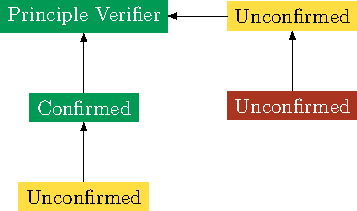
\includegraphics{05 design/assets/verification tree.pdf}
  \caption{Verification Chain}
  \captiondesc{The first two \enquote{unconfirmed}
    employees can
    confirm their verification with the principle verifier
    or
    through the \enquote{confirmed} employee.
    The final \enquote{unconfirmed} employee is attempting to
    confirm with an another unconfirmed employee --- illegal.
  }
  \label{fig:verificationTree}
\end{figure}

Designating the principle verifier can be as simple as
automatically designating the first employee to clock-in;
it could also be pre-configured as a supervisor on-site or
determined programmatically based on employee reliability,
trustworthy, punctuality, etc.